\chapter{Shape and dynamics}
\label{ch:forma}
When it's seen by naked eye, plasma sources for medical uses expel a little plume of plasma that emits radiation in a visible range, with different colours or intensity that depends on the gas composition, it's flow and intensity of applied electric field. 
However if we see this plasma at a specific time, recent studies shows that what is expelled is not a continuos flow, but the ``plume'' is formed by compact bullets with high velocities (\cite{Mericam_Bourdet_2009}, \cite{doi:10.1002/ppap.200900078}).
An example of this phenomenon is shown in figure \ref{fig:pl_bullet}, measured with the experimental apparatus that will be explained later.
\begin{figure}
 \centering
 \includegraphics[width=0.8\textwidth]{Images/Shape/frames.png}
 \caption{Example of plasma bullet expulsion, as measured with our experimental setup, with an helium flow of \SI{2}{\liter/\minute}.}
 \label{fig:pl_bullet}
\end{figure}

Plasma bullets still needs to be studied in depth, we only know the basic dynamic of formation and expulsion. Some general features are that:
\begin{itemize}
 \item bullet's velocities are $> \SI{10}{\kilo\meter/\second}$;
 \item bullet formation, it's velocity and it's travel distance depend on applied tension on the electrode;
 \item frontal image of the bullet, on a plane perpendicular to it's velocity, is not a full circle but it's donut shaped, with an outer ring of higher intensity.
\end{itemize}

The scope of this experiment is to observe plasma bullets produced with our source, their shape and their velocity and how they change with different discharge conditions.

Given their typical velocities and the temperature of the plasma, bullet propagation is tought to be related to a travelling ionization front. This propagation can be studied with simplified simulation of DBD discharges, where it's reproduced the behaviour of plasma bullets (\cite{doi:10.1063/1.4963115}, \cite{Breden_2012}) or the interaction between plasma and a target (\cite{doi:10.1063/1.4923345}).
%We present a simple 1D model that can reproduce the propagation of this ionization front.

\section{Experimental setup}
To visually observe dynamics of plasma formation and propagation, it is needed an acquisition setup with an high-speed camera that has little integration time, around \SI{10}{\nano\second}, and an image intensifier that permits to visualize light emitted in such a short time interval.

This is a measure where we need coincidence between discharge and frame measure so it is necessary to consider instruments and plasma source specific delays and give appropriate triggers.

Experimental setup is shown in photo \ref{fig:fotosetup} and a scheme is presented in \ref{fig:schemashape}, there are the trigger signal lines, optical acquisition pointed at source exit and measure acquisition composed by a computer and an oscilloscope. 
\begin{figure}
 \centering
 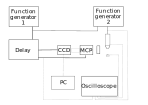
\includegraphics[width=0.6\textwidth]{Images/Shape/acq_ottica.png}
 \caption{Photo of the experimental setup.}
 \label{fig:fotosetup}
\end{figure}

\begin{figure}
 \centering
 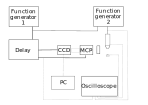
\includegraphics[width=0.7\textwidth]{Images/Shape/acq_ottica.png}
 \caption{Experimental setup scheme. Function generator 1, function generator 2 and delay generator send trigger signal to camera (CCD), to source and to image intensifier (MCP), full lines in the scheme. Camera sends measured frame to a computer (PC) and from source, source's target, function generator 2 and delay are taken signals read on the oscilloscope, pointed lines in the scheme.}
 \label{fig:schemashape}
\end{figure}



\subsection{Source and optical setup}
Source head is positioned vertically and emitted light is collected from the side.
Optical apparatus is composed by a lens %specific
 coupled with a Micro Channel Plate image intensifier (MCP). An MCP works as in figure \ref{fig:MCP}: for every photon received, thanks to an high-voltage power supply, it emits many photons with little angular deviation.
\begin{figure}
 \centering
 \includegraphics[width=0.4\textwidth]{Images/Shape/MCPsingle-stage.jpg}
 \caption{Micro Channel Plate image intensifier functioning.}
 \label{fig:MCP}
\end{figure}

Those photons are received by an high-speed camera \emph{Point Grey Flea} (\cite{flea}) equipped with a CCD of $\num{1024} \times \num{768}$ square pixels $\SI{4.75}{\micro\meter}$ wide. Every frame is sent to the pc where FLIR software elaborates and saves them in pgm format (\cite{pgm}).

\subsection{Source, power lines and electric signals}
It's used a source with electric features and functioning similar to those described before, with an output between $\num{3}$ and \SI{8}{\kilo\volt}, variabile changing $\Delta t$ of the trigger signal (see \ref{ch:electric}), that is always given through an optical fiber with frequency $f$. Differances are that tension is positive and not negative, because it helps formation of the plume with gasses harder to ignite (e.g. Argon), and that trigger signal is given by a generator function ($2$ in the scheme) to define discharge time respect to the trigger of other instruments.

The source is positioned vertically at a distance of \SI{42.0(1)}{\milli\meter} from optical bench, with the glass nozzle that permits to observe plasma formation inside it (external diameter \SI{8.0(1)}{\milli\meter}, internal diameter \SI{6.0(1)}{\milli\meter}), with a distance from the end of the electrode to nozzle exit of \SI{12}{\milli\meter}. At the exit the nozzle shrinks for \SI{3.0(1)}{\milli\meter}, until a diameter of \SI{5.0(1)}{\milli\meter}

Under the source is possible to put targets. Are used two different targets at different heights: conductive target and insulator target. The first one is a copper square sheet of dimensions $\SI{10}{\milli\meter} \times \SI{10}{\milli\meter} \times \SI{1}{\milli\meter}$ (used for current measures in chapter \ref{ch:electric}), the second one is a simple plastic material.


CCD camera is powered by a simple alimentator while image intensifier MCP is powered by an high-voltage supply, both are triggered by the delay generator, with different times (see next section).


On an oscilloscope are measured the trigger signal given to source head, the trigger signal given to MPC, the voltage electrode with high-voltage probe \emph{Tektronix P6015A} and the current intensity when it's used the conductive target. Current intensity measure is done measuring voltage drop on a resistance of $\SI{1}{\mega\ohm}$ with a probe $x\num{10}$.

\subsection{Trigger synchronization}
Experiment's scope is to know plasma dynamics at a specific point on voltage waveform, so it's necessary to know precisely discharge and measure times.

To compose the necessary trigger line are utilized:
\begin{itemize}
 \item function generator \emph{Or-x 310}, $1$ in figure, that sends a square wave with set amplitude, width and frequency $f$;
 \item function generator \emph{Lecroy 9210}, $2$ in figure, that sends a square wave with frequency given by the trigger, amplitude set, and variable width $\Delta t$;
 \item delay time generator \emph{Stanford DG535}, that sends square wave with set amplitude, frequency given by the voltage input and starting times given by voltage input startin time plus settable delays (4 channels).
\end{itemize}

Every intrument has it's own time that elapse between trigger signal and effective measure. The longer one is arming time for high-speed camera in the order of \si{\milli\second}, the smaller one is integration time for acquisition system, that starts from the activation of the image intensifier and span $\SI{15}{\nano\second}$.

A time line is shown in figure \ref{fig:times}, an example of signal taken with the oscilloscope is in figure \ref{fig:times_signals}. There are three relevant times defined by function and delay generators:
\begin{enumerate}
 \item $t_{0}$ is the starting time for the square wave given by \emph{Function generator 1}, with an amplitude of $\SI{5}{\volt}$ and a frequency $f$, that goes as external trigger to \emph{Function generator 2} and as voltage input to \emph{Delay generator}. From \emph{Function generator 2}, at $t_{0}$, starts the square wave that triggers discharge, with a width of $\Delta t$ that will define voltage amplitude (see chapter \ref{ch:electric}) and the same frequency $f$. From \emph{Delay generator}, at $t_{0}$, without delays, starts the trigger signal to arm the camera with the CCD.
 \item $t_{\text{DIS}}$ is the effective discharge time, when the amplitude peak starts. From trigger signal end to amplitude peak start there is a time delay given mainly by the response time of photodiode. Measuring the signals as in figure \ref{fig:times_signals}, it's possible to estimate this delay as $\SI{987.7(567)}{\nano\second}$, constant for every $f$ and $\Delta t$. Once the discharge starts, in the grey zone in figure, there are the events that we want to measure, plasma formation and propagation.
 \item $t_{\text{MIS}}$ is the measure time, when the MCP is triggered on. The delay between $t_{0}$ and $t_{\text{MIS}}$, $t_{D}$, is given by the \emph{Delay generator} with possible steps of \SI{1}{\pico\second}. Changing $t_{D}$ during measure it's possible to see plasma dynamics at different times that corresponds to different points on electrode tension waveform, as in figure \ref{fig:times_signals}.
\end{enumerate}
\begin{figure}
 \centering
 \includegraphics[width=0.6\textwidth]{Images/Shape/times.png}
 \caption{Time signal synchronization scheme: $t_{0}$ is the starting trigger time, $\Delta t$ is the opening time for plasma source (see chapter \ref{ch:electric}), $t_{\text{DIS}}$ is the starting time for the discharge and $t_{\text{MIS}}$ the starting time for the MCP i.e. the measure time}.
 \label{fig:times}
\end{figure}

\begin{figure}
 \centering
 \includegraphics[width=0.6\textwidth]{Images/Shape/times_osc.png}
 \caption{Oscilloscope measure example, in green the discharge trigger, in red the electrode tension output and in blue the MCP trigger.}
 \label{fig:times_signals}
\end{figure}


Integration time for a single frame is \SI{15}{\nano\second}, so the time step between two measures has to be larger then it. For slow plasma bullets (Neon or Argon) it's used a step of \SI{50}{\nano\second}, for fast bullets (Helium) it's used a step of \SI{20}{\nano\second}.


The effective measure time have to consider slower time of the camera, larger then \SI{50}{\milli\second}. It's important to note that also with little frequencies, around \SI{50}{\hertz} (see later the minimum working frequency for different gasses), time between two pulses is \SI{20}{\milli\second}, so it is not possible to see two consecutive frames, we observe the same time in different discharges.

Changing the settings on camera acquisition software is possible to measure a signal below pixel's saturation point. One of the parameters is the \emph{Shutter time}, the opening time of the camera shutter, that if set on a value larger then the time between two signals permits to integrate between two frames.
When we work with a gas, we select an appropriate \emph{Gain} value and an appropriate \emph{Shutter time}, chosing to work measuring a single discharge frame or a multiple discharge frame.

\subsection{Different setups}
Plasma formation is influenced by many parameters such as frequency of high-voltage pulses, their rise time and maximum, gas type, gas flow, presence of a target and its features (see \cite{Mericam_Bourdet_2009}, \cite{Jarrige_2010}).

For pulse frequency we find a lower limit value, different for each ignition gas, under which there is no discharge. For frequencies higher then this value we don't expect changes (as there aren't in the electric behaviour in chapter \ref{ch:electric}), so we use a single chosen value that permits plasma ignition and doesn't stress the experimental setup.
High-voltage values and gas type determine plasma bullet formation and affect its expulsion velocity. In particular, different gasses have different atomic mass and ionization energies, they will have different voltage ignition values and reactive species formed in plasma will have different velocities.
Gas flow influences how much gas there is when the ignition starts, so varying it we observe different bullets diameter and velocity.
Target influences bullet expulsion, propagation and plasma rebound signal. With a conductive target near plasma exit we will have an easier path seen by charges that propagates and, once the bullet hits the target, its observed higher luminosity going from the target to the electrode. With an insulator target we don't find the ionization channel closing on the target, but we observe charge deposition on the insulator with a shape that depends from the gas and the target.
In some setups, to help plasma ignition it's also used a conductor ring at ground potential or at floating potential, placed around source nozzle, after the electrode position.


In this study we present different setups with three different gasses, as shown in table \ref{tab:setups}.

\begin{table}
 \centering
 \begin{tabular}{cccccccc}
  \toprule
  Gas   &Setup  &$\Delta t$ &Target &Target position    &Flow rate  &Other  &$\Delta t_D$\\
  \midrule
  \multirow{8}*{\ce{He}}    &A  &$\num{30}, \num{35}, \num{40}$ &Conductor  &\SI{24}{\milli\meter}  &\SI{2}{\liter/\minute} &-  &\SI{50}{\nano\second}\\
                            &B  &$\num{30}, \num{35}, \num{40}$ &Conductor  &\SI{32}{\milli\meter}  &\SI{2}{\liter/\minute} &-  &\SI{20}{\nano\second}\\
                            &C  &$\num{30}, \num{35}, \num{40}$ &Insulator  &\SI{24}{\milli\meter}  &\SI{2}{\liter/\minute} &-  &\SI{20}{\nano\second}\\
                            &D  &$\num{30}, \num{35}, \num{40}$ &-  &-  &\SI{2}{\liter/\minute} &-  &\SI{20}{\nano\second}\\
                            &E  &$\num{35}$ &-  &-  &\SI{2}{\liter/\minute} &Ground ring  &\SI{20}{\nano\second}\\
                            &F  &$\num{35}$ &-  &-  &\SI{1}{\liter/\minute} &-  &\SI{20}{\nano\second}\\
                            &G  &$\num{35}$ &-  &-  &\SI{3}{\liter/\minute} &-  &\SI{20}{\nano\second}\\
                            &H  &$\num{35}$ &-  &-  &\SI{4}{\liter/\minute} &-  &\SI{20}{\nano\second}\\
  \midrule
  \multirow{5}*{\ce{Ne}}    &A  &$\num{20}, \num{25}, \num{30}$ &Conductor  &\SI{24}{\milli\meter}  &\SI{2}{\liter/\minute} &-  &\SI{50}{\nano\second}\\
                            &B  &$\num{20}, \num{25}, \num{30}$ &Conductor  &\SI{32}{\milli\meter}  &\SI{2}{\liter/\minute} &-  &\SI{50}{\nano\second}\\
                            &C  &$\num{20}, \num{25}, \num{30}$ &Insulator  &\SI{24}{\milli\meter}  &\SI{2}{\liter/\minute} &-  &\SI{50}{\nano\second}\\
                            &D  &$\num{20}, \num{25}, \num{30}$ &-  &-  &\SI{2}{\liter/\minute} &-  &\SI{50}{\nano\second}\\
                            &E  &$\num{30}$ &-  &-  &\SI{2}{\liter/\minute} &Ground ring  &\SI{50}{\nano\second}\\
  \midrule
  \multirow{6}*{\ce{Ar}}    &A  &$\num{35}$ &-  &-  &\SI{2}{\liter/\minute} &Ground ring  &\SI{50}{\nano\second}\\
                            &B  &$\num{35}$ &-  &\SI{32}{\milli\meter}  &\SI{2}{\liter/\minute} &-  &\SI{20}{\nano\second}\\
                            &C  &$\num{35}$ &-  &-  &\SI{2}{\liter/\minute} &Floating ring  &\SI{50}{\nano\second}\\
                            &D  &$\num{35}$ &Conductor  &\SI{20}{\milli\meter}  &\SI{2}{\liter/\minute} &Ground ring  &\SI{50}{\nano\second}\\
                            &E  &$\num{35}$ &Conductor  &\SI{20}{\milli\meter}  &\SI{2}{\liter/\minute} &-  &\SI{50}{\nano\second}\\
                            &F  &$\num{35}$ &-  &-  &\SI{2}{\liter/\minute} &-  &\SI{50}{\nano\second}\\
                            &G  &$\num{35}$ &Conductor  &\SI{32}{\milli\meter}  &\SI{2}{\liter/\minute} &-  &\SI{50}{\nano\second}\\
  \bottomrule
 \end{tabular}
 \caption{Description of measure setups. In first column there is the gas; second column is the setup name; third column is voltage pulse time width, expressed as percentage of a square trigger \SI{10}{\micro\second} long; four and fifth columns are target information, where it's used a target; sixth column is used gas flow; seventh column are other informations, i.e. if it's used the conductor ring explained before; eight column is the time step between two different frames.}
 \label{tab:setups}
\end{table}


\subsection{Frame analysis and calibration}
Once a measure setup is chosen, $t_D$ is set around the start of the discharge, we measure the oscilloscope waveform for every channel (setup as explained before), and from them we save $5$ frames for every $t_D$ varying it with steps of $\Delta t_D$. Measures are taken until the end of the main tension peaks and the camera doesn't see anything.


From oscilloscope waveforms we can extrapolate the measure time from the start of the discharge and tension value at measure time. When there is the conductive target it's also possible to see current intensity and it's peak time.


Frame analysis is done converting the pgm files in 2-dimensional histograms, using \emph{TH2} class written in \emph{ROOT} libraries (see \cite{ROOT:TH2}).
We are interested in plasma bullet formation and it's expulsion, but also in other fenomenological behaviour that is observed during measures.

For plasma bullet we take the mean for every pixel between the five frames taken, from then it's isolated the plasma bullet as the collection of pixels with maximum intensity in the frame. From this image we extrapolate the position of the bullet with the coordinates of it's luminosity barycenter on the plane seen by camera, called x-y in the analysis.
Once established the center, we can find it's contour as the points were luminosity goes under a certain percentage of the maximum, from that we estimate it's dimensions along x and y axis and it's average luminosity.
With barycenter coordinates it's possible to compute their velocity using a finite differance formula (that takes into consideration possible different time steps, see \cite{Bhadauria}).


Actual dimensions on a frame are found with a calibration with a known target: it is used a plate with $4$ holes, diameter of \SI{1.0(1)}{\milli\meter} at the vertice of a square with an edge lenght of \SI{10.0(1)}{\milli\meter}, positioned at plasma exit (source is off) and illuminated from behind with a torch.
Acquiring a frame of this setup it's possible to extrapolate pixel's distance that corresponds to \SI{10}{\milli\meter} for every square edge, average them, and calculate pixel's width in our frames, resulting a value of $d_{pix} = \SI{0.172(2)}{\milli\meter}$.

\section{Helium flow}
We start the presentation of measures with helium, as it is commonly used for medical applications of plasma.
Helium it's an element with standard atomic weight of $\num{4.002}$, 1st ionization energy of \SI{24.587}{\electronvolt} and 2nd ionization energy of \SI{54.418}{\electronvolt}.
It's easy to produce helium plasma, when it's ignited it emits radiation with principal wavelenghts in violet and orange ($\lambda = \num{388.86}$ and \SI{587.56}{\nano\meter}), resulting in a purple plume at naked eye.
Principal downside of helium gasses it's that they are expensive.


In our experiment we produce helium plasma with pulse frequency $f = \SI{5}{\kilo\hertz}$ and $\Delta t = \num{3}$, $\num{3.5}$ and \SI{4}{\micro\second}, as explained in table \ref{tab:setups}.
Delays are setted to take a single frame during every acquisition, for every measure we take $5$ frames and average them.


First we present a tipical discharge without target, after is shown how the behaviour changes varying parameters and then it's discussed how a target influences bullet propagation.

\subsection{Plasma bullet description}
We use as example bullet the setup D with $\Delta t = \SI{3.5}{\micro\second}$, i.e. absence of a target and gas flow of \SI{2}{\liter/\minute}.


It's possible to divide the phenomenon that we want to observe in four phases, as presented in figure \ref{fig:bullet_es}: bullet formation, bullet displacement inside the nozzle, bullet expulsion and bullet propagation outside the nozzle, in air. It's important to remember that time values goes from the start of the voltage peak, extrapolated from oscilloscope measures.
When the voltage goes over a definite value, we observe a rapid increase in luminosity around the electrode that it's interpreted as plasma formation. From there, in a time of $\sim \SI{50}{\nano\second}$ the plasma modifies it'shape and becames what we call the bullet: a zone with high luminosity confined in space. The bullet then moves in the exit direction and it's expelled always with a well defined front. In air we see the round shaped bullet propagation, until it reaches a maximum travel distance and then luminosity decreases rapidly, until we see nothing more. In these measure conditions we see again plasma formation in correspondence of the negative tension peak, but it is  a rapid process without propagation.
\begin{figure}
 \centering
 \subfloat[\SI{140.93}{\nano\second}]{
    \includegraphics[width=0.48\textwidth]{Images/Shape/elio_d035_es1.png}
 }
 \hfill
 \subfloat[\SI{240.93}{\nano\second}]{
    \includegraphics[width=0.48\textwidth]{Images/Shape/elio_d035_es2.png}
 }
 
 \subfloat[\SI{400.93}{\nano\second}]{
    \includegraphics[width=0.48\textwidth]{Images/Shape/elio_d035_es3.png}
 }
 \hfill
 \subfloat[\SI{460.93}{\nano\second}]{
    \includegraphics[width=0.48\textwidth]{Images/Shape/elio_d035_es4.png}
 }
 \caption{Four phases of plasma dynamics: bullet formation (a), bullet displacement inside the nozzle (b), bullet expulsion (c) and bullet propagation outside the nozzle (d). Time intervals are calculated from the start of the voltage peak.}
 \label{fig:bullet_es}
\end{figure}


\paragraph{Electrode voltage and bullet intensity}
The time interval in wich we see the bullet can be defined as where we can see a definite zone with mean luminosity higher then the background. The starting time is given by voltage reaching a certain value, when we see bullet formation, and the bullet expires when it's luminosity decreases.

In figure \ref{fig:elio_d035_I} are presented the mean intensity of the plume during the motion and the zoom on the intersted time interval for voltage measure. Plasma formation is observed around \SI{120.93}{\nano\second} after peak start, at a tension value of \SI{5710.00(28550)}{\volt}. %while maximum peak value is \SI{6588.80(32944)}{\volt} at time \SI{260.93}{\nano\second}.
As we can see, luminosity is higher during plasma formation around the electrode and it decrease very little during all the propagation, even after the expulsion in air (pointed line on the graph). After a time of \SI{440}{\nano\second} the bullet luminosity decreases rapidly and it disperses in the air.
\begin{figure}
 \centering
 \subfloat[Zoom on voltage waveform.]{
    \includegraphics[width=0.48\textwidth]{Images/Shape/elio_d035_V.png}
 }
 \hfill
 \subfloat[Mean intensity of plasma bullet.]{
    \includegraphics[width=0.48\textwidth]{Images/Shape/elio_d035_Im.png}
 }
 \caption{Voltage waveform and intensity of the bullet versus time. Time zero is the start of the voltage peak, ending time is taken as the time where intensity reaches background value. The pointed line in intensity graph indicates the end of the nozzle.}
 \label{fig:elio_d035_I}
\end{figure}

\paragraph{Barycenter coordinates and direction}
The motion of the bullet on observing plane can be extrapolated from it's barycenter coordinates.

In figure \ref{fig:elio_d035_bary} there are the two coordinates versus time.
Coordinate x, along the axis of the source (of the electrode and the nozzle) is more relevant to observe bullet expulsion. We see as plasma forms around position $\SI{73}{\milli\meter}$ and the nozzle ends at $\SI{85}{\milli\meter}$, compatible with the distance electrode-nozzle exit described before. After plasma formation we can see bullet displacement in the nozzle with a certain velocity, until it reaches the exit and propagates in the air more rapidly. The bullet travels until it reaches a maximum x, covering a distance of \SI{26.08(2)}{\milli\meter} from the electrode. It seems that the bullet stops while it's luminosity decreases.

Coordinate y it's relevant to show bullet direction, as we can see, it moves in a space interval of \SI{2}{\milli\meter}. The bullet forms over the electrode, then, when it enlarges to cover all the nozzle diameter, lowers it's barycenter with a constant slope, even after the expulsion. Once the bullet starts to decrease in luminosity, it stops its motion also on the y direction.
\begin{figure}
 \centering
 \subfloat[]{
    \includegraphics[width=0.48\textwidth]{Images/Shape/elio_d035_xb.png}
 }
 \hfill
 \subfloat[]{
    \includegraphics[width=0.48\textwidth]{Images/Shape/elio_d035_yb.png}
 }
 \caption{Barycenter coordinates of the bullet. Pointed lines indicate the end of the nozzle.}
 \label{fig:elio_d035_I}
\end{figure}

Lowering of the baricenter in the y direction it's explainable by a tilt in the source, that is not perfectly perpendicular to the optical bench, if we consider the entire dimension of the bullet in the y direction, with it's upper and lower limits. In figure \ref{fig:elio_d035_diry} are shown y maximum, minimum and baricenter of the bullet, in function of the x brycenter coordinate and can be seen how the entire figure points downward (to the side turning the image). Inside the nozzle we can take y maximum as a value that defines the contour of the nozzle, with a fit as in figure we find a value of \SI{3.39(10)}{\degree}. Outside the nozzle we find that the barycenter direction is pointed \SI{3.71(4)}{\degree} downward, a little higher then the direction of the nozzle. The values are almost compatible with each other, so it seems to suggest that tilting the source it's possible to direct the bullet even after it's propagation in air.
\begin{figure}
 \centering
 \includegraphics[width=0.6\textwidth]{Images/Shape/elio_d035_incl.png}
\end{figure}


\paragraph{Bullet dimensions}
Once we define the contour of the bullet, it's simple to take it's dimensions along the two directions.

In figure \ref{fig:elio_d035_dim} are presented width and height of the bullet.
In the x direction, the bullet presents constant diameter until it approaches nozzle exit, where it enlarges a little to reach the exit. In the air the bullet mantaines its dimension, with values a little lower then inside the nozzle, but compatible within the error. When it stops it seems to have greater diameter, but the measure loses significance as the bullet fades in the air and it can be confused with the background.
In y direction we find a constant value of \SI{4.65(20)}{\milli\meter} during propagation in the nozzle, as expected because the bullet covers all the nozzle area, a little lower then its diameter due to glass refraction effects. Once the nozzle shrinks, the bullet diminish it's diameter and maintains a constant value of \SI{2.07(20)}{\milli\meter} during all the propagation in air, until it stops.
\begin{figure}
 \centering
 \subfloat[]{
    \includegraphics[width=0.48\textwidth]{Images/Shape/elio_d035_dx.png}
 }
 \hfill
 \subfloat[]{
    \includegraphics[width=0.48\textwidth]{Images/Shape/elio_d035_dy.png}
 }
 \caption{Dimensions of the bullet. Pointed lines indicate the end of the nozzle.}
 \label{fig:elio_d035_I}
\end{figure}


\paragraph{Bullet velocity}
From barycenter graphs we see as bullet motion has a definite velocity during described phases.
Fitting the graph with a line during the displacement phase inside the nozzle, as in figure \ref{fig:elio_d035_vx}, we find that it moves with a speed of $v_{N} = \SI{46.48(20)}{\kilo\meter/\second}$. Once it exits the nozzle it speeds up, until a value of $v_{A} = \SI{95.16(60)}{\kilo\meter/\second}$.


With a 3 point finite differance formula we can estimate it's velocity point by point (excluding the first and the last), finding the values shown in figure \ref{fig:elio_d035_vx}. From those values we can average velocities during the two motion phases, finding compatible mean value respect the linear fit: $v_{N} = \SI{48.23(103)}{\kilo\meter/\second}$ and $v_{A} = \SI{95.16(182)}{\kilo\meter/\second}$.
\begin{figure}
 \centering
 \subfloat[Fit of x barycenter.]{
    \includegraphics[width=0.48\textwidth]{Images/Shape/elio_d035_xb_fitv.png}
 }
 \hfill
 \subfloat[Velocities in x direction.]{
    \includegraphics[width=0.48\textwidth]{Images/Shape/elio_d035_vx_fitv.png}
 }
 \caption{Velocity of the bullet in x direction. Pointed lines indicate the end of the nozzle, red lines calculated values during displacement and propagation phases.}
 \label{fig:elio_d035_vx}
\end{figure}

It's interesting to point out that those velocities are much higher then the average velocity of the neutral gas, that for a flow of \SI{2}{\liter/\minute} is of \SI{12}{\meter\second}.

\subsection{Voltage influence}
With an higher $\Delta t$ we can reach higher voltage peak values (see chapter \ref{ch:electric}), so we will have higher electron energies. With more energy we expect that the bullet will reach furter distances, with higher velocity. In figure \ref{fig:elio_d} and table \ref{tab:elio_d} are presented the results of the analysis.

The discharge starts always in the same voltage interval, around \SI{5.7}{\kilo\volt}. We observe a higher luminosity with higher tensions, but it decreases always in a time interval around \SI{100}{\nano\second} once it exits the nozzle (figure \ref{fig:elio_d} (a)).

The plot for the barycenter coordinates (figure \ref{fig:elio_d} (b) - (c)) shows how with higher voltage the bullet reaches further distances ($x_{\text{dist}}$ and $y_{\text{dist}}$ in table). For the lower voltage peak it seems that the bullet doesn't propagate in air, as it stops right after nozzle exit.

Dimensions of the bullet (figure \ref{fig:elio_d} (d) - (e)) are not influenced by voltage value, as we can see they have the exact same behaviour, around the same values, for every opening time. A notable differance it's in the y diameter inside the nozzle, where for higher tension we have a slightly larger value. As mentioned before here we have refraction effects due to the glass nozzle, different for those measures due to the higher luminosity.

Velocity values (figure \ref{fig:elio_d} (f)) show how the bullet behaviour is solid during the propagation inside the nozzle and becames more erratic once it exits. As mentioned before, for the lowest opening time we have lower velocities and a rapid drop after contact with air, in this configuration it's not possible to find a propagation velocity. For higher opening times we find the same behaviour, with a proportionality between peak voltage value and velocities: if before we found a stable motion with $v_{A} = \SI{92.93(6)}{\kilo\meter/\second}$, with higher tension it reaches $v_{A} = \SI{149.47(9)}{\kilo\meter/\second}$.

\begin{figure}
 \centering
 \subfloat[Mean luminosity.]{
    \includegraphics[width=0.48\textwidth]{Images/Shape/elio_d_Im.png}
 }
 \hfill
 \subfloat[x barycenter.]{
    \includegraphics[width=0.48\textwidth]{Images/Shape/elio_d_xb.png}
 }
 \subfloat[y barycenter.]{
    \includegraphics[width=0.48\textwidth]{Images/Shape/elio_d_yb.png}
 }
 \hfill
 \subfloat[x diameter.]{
    \includegraphics[width=0.48\textwidth]{Images/Shape/elio_d_dx.png}
 }
 \subfloat[y diameter.]{
    \includegraphics[width=0.48\textwidth]{Images/Shape/elio_d_dy.png}
 }
 \hfill
 \subfloat[x velocity.]{
    \includegraphics[width=0.48\textwidth]{Images/Shape/elio_d_vx.png}
 }
 \caption{Results of the analysis for setup d (helium flow of \SI{2}{\liter/\minute} without target), with different peak voltage values.}
 \label{fig:elio_d}
\end{figure}

\begin{comment}
\begin{table}
 \centering
 \begin{tabular}{ccccccc}
 \toprule
 $V_{p}$ [kV]    &$t_{0}$ [ns] &$V_{0}$ [kV]    &$x_{\text{dist}}$ [mm]   &$y_{\text{dist}}$ [mm]   &$v_{N}$ [km/s]   &$v_{A}$ [km/s]\\
 \midrule
 \num{5.66(30)}  &\num{131.5}  &\num{5.55(28)}    &\num{15.99(1)} &\num{1.66(2)}  &\num{37.72(4)} &-\\
 \num{6.59(33)}  &\num{120.9}  &\num{5.71(29)}    &\num{26.08(2)} &\num{1.92(4)}  &\num{46.48(2)} &\num{95.16(6)}\\
 \num{7.22(36)}  &\num{119.5}  &\num{6.01(30)}    &\num{34.55(5)} &\num{2.07(1)}  &\num{59.80(3)} &\num{149.47(9)}\\
 \bottomrule
 \end{tabular}
 \caption{Result of the analysis with different voltage peak values for the pulse. $V_{p}$ is the peak value for the pulse, $t_{0}$ bullet formation time, $V_{0}$ bullet formation tension, $x_{\text{dist}}$ and $y_{\text{dist}}$ are the highest distances reached by the bullet from electrode position, $v_{N}$ is the velocity in x direction reached inside the nozzle, $v_{A}$ is the velocity of propagation in air in x direction.}
 \label{tab:elio_d}
\end{table}
\end{comment}

\begin{table}
 \centering
 \begin{tabular}{cccccc}
 \toprule
 $V_{p}$ [kV]    &$V_{0}$ [kV]    &$x_{\text{dist}}$ [mm]   &$y_{\text{dist}}$ [mm]   &$v_{N}$ [km/s]   &$v_{A}$ [km/s]\\
 \midrule
 \num{5.66(30)}  &\num{5.55(28)}    &\num{15.99(1)} &\num{1.66(2)}  &\num{37.72(4)} &-\\
 \num{6.59(33)}  &\num{5.71(29)}    &\num{26.08(2)} &\num{1.92(4)}  &\num{46.48(2)} &\num{95.16(6)}\\
 \num{7.22(36)}  &\num{6.01(30)}    &\num{34.55(5)} &\num{2.07(1)}  &\num{59.80(3)} &\num{149.47(9)}\\
 \bottomrule
 \end{tabular}
 \caption{Result of the analysis with different voltage peak values for the pulse. $V_{p}$ is the peak value for the pulse, $V_{0}$ bullet formation tension, $x_{\text{dist}}$ and $y_{\text{dist}}$ are the highest distances reached by the bullet from electrode position, $v_{N}$ is the velocity in x direction reached inside the nozzle, $v_{A}$ is the velocity of propagation in air in x direction.}
 \label{tab:elio_d}
\end{table}


\subsection{Flow influence}
As said before, neutral gas velocity is very little in comparision of the ionization front velocity of the bullet, we expect that changes in the gas flow will have an effect on the quantity of helium present in the nozzle more then on the energy of the atoms and electrons. We try four different flows with the same peak voltage, in figure \ref{fig:elio_d} and table \ref{tab:elio_d} are presented the results of the analysis.

Also for this parameter, the discharge starts always in the same voltage interval, around \SI{5.7}{\kilo\volt}. For gas flows of $\num{1}$ and \SI{2}{\liter/\minute} bullet luminosity decreases in a time interval around \SI{100}{\nano\second} once it exits the nozzle, for higher flows it has a luminosity clearly stronger then background for a longer time interval, around \SI{200}{\nano\second} (figure \ref{fig:elio_035} (a)).

From the barycenter coordinates (figure \ref{fig:elio_d} (b) - (c)) we see as more gas flow seems to be correlated with lower mobility of the bullet: we have shorter distances with higher flows. For maximum tried flow, even if bullet luminosity is more then the background, the bullet travels a very little distance from the exit of the nozzle and it's barycenter remains almost fixed in space.

Dimensions of the bullet (figure \ref{fig:elio_d} (d) - (e)) are not very  influenced by gas flow, but we can see little inverse proportionality. For stronger flows we have always littler diameters inside the nozzle, in both directions.

Velocities shows how the bullet behaviour changes also inside the nozzle varying gas flow (figure \ref{fig:elio_d} (f)). With little flow, we find a costant displacement velocity in the nozzle, while with more flow the bullet slows down when moving (as shown in \cite{Jarrige_2010}), with a decrease in velocity of \SI{7.58(4)}{\kilo\meter/\second/\milli\meter}.
Once the bullet exits the nozzle, we see how it almost stops when there is high flow, while it shows the same behaviour if flow is under \SI{3}{\liter/\minute} and it has maximum velocity for the lowest gas flow, maintaining it for longer time.


Can be concluded that with higher flow we have bullet with longer lifetime and littler mobility, reaching lesser distances with lesser velocity.


\begin{figure}
 \centering
 \subfloat[Mean luminosity.]{
    \includegraphics[width=0.48\textwidth]{Images/Shape/elio_035_Im.png}
 }
 \hfill
 \subfloat[x barycenter.]{
    \includegraphics[width=0.48\textwidth]{Images/Shape/elio_035_xb.png}
 }
 \subfloat[y barycenter.]{
    \includegraphics[width=0.48\textwidth]{Images/Shape/elio_035_yb.png}
 }
 \hfill
 \subfloat[x diameter.]{
    \includegraphics[width=0.48\textwidth]{Images/Shape/elio_035_dx.png}
 }
 \subfloat[y diameter.]{
    \includegraphics[width=0.48\textwidth]{Images/Shape/elio_035_dy.png}
 }
 \hfill
 \subfloat[x velocity.]{
    \includegraphics[width=0.48\textwidth]{Images/Shape/elio_035_vx.png}
 }
 \caption{Results of the analysis for different gas flow (opening time of \SI{3.5}{\micro\second} without target).}
 \label{fig:elio_d}
\end{figure}

\begin{comment}
\begin{table}
 \centering
 \begin{tabular}{ccccccc}
 \toprule
 Flow [L/min]    &$t_{0}$ [ns] &$V_{0}$ [kV]    &$x_{\text{dist}}$ [mm]   &$y_{\text{dist}}$ [mm]   &$v_{N}$ [km/s]   &$v_{A}$ [km/s]\\
 \midrule
 \num{1}  &\num{121.9}  &\num{5.87(8)}    &\num{30.65(3)} &\num{2.75(1)}  &\num{54.33(10)} &\num{113.97(9)}\\
 \num{2}  &\num{120.9}  &\num{5.71(29)}    &\num{26.08(2)} &\num{1.92(4)}  &\num{46.48(2)} &\num{95.16(6)}\\
 \num{3}  &\num{124.0}  &\num{5.41(27)}    &\num{19.38(1)} &\num{1.84(1)}  &\num{39.88(4)} &\num{40.96(10)}\\
 \num{4}  &\num{121.3}  &\num{5.90(12)}    &\num{22.80(3)} &\num{2.30(1)}  &\num{58.89(14)} &\num{61.94(44)}\\
 \bottomrule
 \end{tabular}
 \caption{Result of the analysis with different gas flows. $t_{0}$ is the bullet formation time, $V_{0}$ the bullet formation tension, $x_{\text{dist}}$ and $y_{\text{dist}}$ are the highest distances reached by the bullet from electrode position, $v_{N}$ is the velocity in x direction reached inside the nozzle, $v_{A}$ is the velocity of propagation in air in x direction.}
 \label{tab:elio_d}
\end{table} 
\end{comment}

\begin{table}
 \centering
 \begin{tabular}{cccccc}
 \toprule
 Flow [L/min]    &$V_{0}$ [kV]    &$x_{\text{dist}}$ [mm]   &$y_{\text{dist}}$ [mm]   &$v_{N}$ [km/s]   &$v_{A}$ [km/s]\\
 \midrule
 \num{1}  &\num{5.87(8)}    &\num{30.65(3)} &\num{2.75(1)}  &\num{54.33(10)} &\num{113.97(9)}\\
 \num{2}  &\num{5.71(29)}    &\num{26.08(2)} &\num{1.92(4)}  &\num{46.48(2)} &\num{95.16(6)}\\
 \num{3}  &\num{5.41(27)}    &\num{19.38(1)} &\num{1.84(1)}  &\num{39.88(4)} &\num{40.96(10)}\\
 \num{4}  &\num{5.90(12)}    &\num{22.80(3)} &\num{2.30(1)}  &\num{58.89(14)} &\num{61.94(44)}\\
 \bottomrule
 \end{tabular}
 \caption{Result of the analysis with different gas flows. $V_{0}$ the bullet formation tension, $x_{\text{dist}}$ and $y_{\text{dist}}$ are the highest distances reached by the bullet from electrode position, $v_{N}$ is the velocity in x direction reached inside the nozzle, $v_{A}$ is the velocity of propagation in air in x direction.}
 \label{tab:elio_d}
\end{table}


\subsection{Insulator target}
Plasma produced with this source will be applied on biological tissues, so it's fundamental to know how bullet behaviour changes with different targets.

An insulator target is not expected to affect the behaviour until the bullet reaches it. An intersting effect is seen after the impact of the bullet with the target, as in figure \ref{fig:elio_ins}, where the plasma seems to deposit charge on the insulator in a circular shape.
\begin{figure}
 \centering
 \subfloat[Bullet propagation \SI{437.6}{\nano\second}.]{
    \includegraphics[width=0.42\textwidth]{Images/Shape/elio_ins1.png}
 }
 \hfill
 \subfloat[Bullet impact \SI{457.6}{\nano\second}.]{
    \includegraphics[width=0.42\textwidth]{Images/Shape/elio_ins2.png}
 }
 \hfill
 \subfloat[Charge deposition \SI{577.6}{\nano\second}.]{
    \includegraphics[width=0.42\textwidth]{Images/Shape/elio_ins3.png}
 }
 \caption{Impact and charge deposition on an insulator target.}
 \label{fig:elio_ins}
\end{figure}


In figure \ref{fig:elio_c_xb} we can see barycenter's x-coordinate of the bullet and its diameter. While for the lowest tension value we see that the bullet stops before it reaches the target, for the other two sets it clearly stops at the target position. Distance values are comparable with those without target (figure \ref{fig:elio_d}), a little higher for medium tension value, as the bullet instead of stopping at a position before it (as it does whitout target) collide with the target.
Bullet width is exactly the same with or without target during it's propagation. We can see changes only when it impacts on the target and shrinks rapidly.
Displacement velocities inside the nozzle and propagation velocities in air are of the same order of values without target, as we can see in figure \ref{fig:elio_c_vx}. We find higher $v_{A}$ only for medium tension value, where it reaches \SI{118.98(7)}{\kilo\meter/\second}, due to the rapid collision with the target instead of slowing down and stopping.
\begin{figure}
 \centering
 \subfloat[Barycenter position.]{
    \includegraphics[width=0.48\textwidth]{Images/Shape/elio_c_xb.png}
 }
 \hfill
 \subfloat[Bullet diameter.]{
    \includegraphics[width=0.48\textwidth]{Images/Shape/elio_c_dx.png}
 }
 \caption{Barycenter motion and diameter in x direction, for different voltage peak values.}
 \label{fig:elio_c_xb}
\end{figure}

\paragraph{Charge deposition}
Once the bullet reaches the target we can see how the glowing region enlarges on its surface from the plot of y diameter, as in figure \ref{fig:elio_c_ylim}. To evaluate the expansion diameter and velocity, we can plot the differance between y limit and y barycenter once the bullet reaches the target. In figure \ref{fig:elio_c_ylim} we can see that the diameter of the maximum expansion is little higher for larger tension value, as well as it's expansion velocity: for opening time of \SI{3.5}{\micro\second} we find a diameter of \SI{6.54(4)}{\milli\meter} and an expansion velocity of \SI{31.36(25)}{\kilo\meter/\second}, while for \SI{4.0}{\micro\second} we find \SI{7.40(2)}{\milli\meter} and \SI{64.04(39)}{\kilo\meter/\second}. It is an expected result as the bullet have more energy with an higher peak value, the velocity along x is larger and we have also higher expansion velocity.

\begin{figure}
 \centering
 \subfloat[Bullet diameter.]{
    \includegraphics[width=0.48\textwidth]{Images/Shape/elio_c_dy.png}
 }
 \hfill
 \subfloat[Bullet expansion in time.]{
    \includegraphics[width=0.48\textwidth]{Images/Shape/elio_c_ylim.png}
 }
 \caption{Bullet expansion in the y direction. We see the absolute value for the diameter for all barycenter positions (a) and a zoom on the expansion for times after it reaches the target (b), where y contour values are calculated as differance with the barycenter y coordinate. Linear fits show how much the diameter enlarges in time.}
 \label{fig:elio_c_ylim}
\end{figure}


\subsection{Distant conductive target}
In measure set A the target is positioned at \SI{24}{\milli\meter} from the bench, correponding to \SI{30}{\milli\meter} from the electrode. A conductive target is expected to affect bullet behaviour as it reachs its proximity, as there are free charges on the surface. If with an insulator we see charge deposition, with a conductor we see a rapid backstream (with a motion inverse to that of the bullet) with great luminosity when the bullet impacts on it, as in figure \ref{fig:elio_met}.
\begin{figure}
 \centering
 \subfloat[Bullet propagation \SI{371.2}{\nano\second}.]{
    \includegraphics[width=0.42\textwidth]{Images/Shape/elio_met1.png}
 }
 \hfill
 \subfloat[Bullet impact \SI{391.2}{\nano\second}.]{
    \includegraphics[width=0.42\textwidth]{Images/Shape/elio_met2.png}
 }
 \hfill
 \subfloat[Backstream \SI{411.2}{\nano\second}.]{
    \includegraphics[width=0.42\textwidth]{Images/Shape/elio_met3.png}
 }
 \caption{Impact and backstream with a copper target.}
 \label{fig:elio_met}
\end{figure}

\paragraph{Bullet dynamics}
Considering only the bullet, separated from the backstream, first thing to note with this target, is how all the system is more reactive to tension values: as we can see in figure \ref{fig:elio_a_Im}, we find that plasma bullet luminosity is enanched in correspondence of the second tension peak (negative), even if it doesn't move from the target as shown in figure \ref{fig:elio_a_xb} (a). Thanks to this second peak, bullet lifetime is longer, it shows luminosity even after \SI{900}{\nano\second} from the start.
\begin{figure}
 \centering
 \subfloat[Voltage waveforms.]{
    \includegraphics[width=0.43\textwidth]{Images/Shape/elio_a_V.png}
 }
 \hfill
 \subfloat[Bullet luminosity.]{
    \includegraphics[width=0.43\textwidth]{Images/Shape/elio_a_Im.png}
 }
 \caption{Voltage applied to the elctrode and bullet luminosity for different measure sets. Note the second luminosity peak in correspondence of the negative voltage peak.}
 \label{fig:elio_a_Im}
\end{figure}


Barycenter motion shows also some peculiarities: even with low tension the bullet reaches the target, showing larger propagation velocity then with other configurations. It's diameter doesn't shows different behaviour, it stays constant until nozzle exit and remains constant until it reaches the target and shrinks to a point. As said before, velocities of propagation in air are generally larger then whitout target, they arrives from \SI{112.04(5)}{\kilo\meter/\second} for low voltage peak to \SI{160.55(9)}{\kilo\meter/\second} for high voltage peak.
\begin{figure}
 \centering
 \subfloat[Barycenter.]{
    \includegraphics[width=0.43\textwidth]{Images/Shape/elio_a_xb.png}
 }
 \hfill
 \subfloat[Diameter.]{
    \includegraphics[width=0.43\textwidth]{Images/Shape/elio_a_dx.png}
 }
 \subfloat[Velocity.]{
    \includegraphics[width=0.43\textwidth]{Images/Shape/elio_a_vx.png}
 }
 \caption{Bullet barycenter coordinate, diameter and velocity along x direction, with copper target. When the bullet reaches the target, it shrinks and stops.}
 \label{fig:elio_a_xb}
\end{figure}


\paragraph{Current measure}
Thanks to the conductive target, we can measure current intensity flowing in it due to charge transported by bullets, and, more intersting, the relation between impact time and when it's measured peak current.
Current intensity it's shown in figure \ref{fig:elio_a_icurr}, we can see a positive peak, more influenced by tension peak value, and a negative peak in correspondence of the negative tension peak and of the second luminosity peak for the bullet. It's important to note that the time interval where we have high luminosity for the bullet and its position is around the target position, is the same time interval where we measure current.
\begin{figure}
 \centering
 \includegraphics[width=0.6\textwidth]{Images/Shape/elio_a_icurr.png}
 \caption{Current intensity measured in set A, with different voltage peak values.}
 \label{fig:elio_a_icurr}
\end{figure}

In the graphs we can distinguish a starting time for the peak current, and a time where it reaches it's maximum value. Even if it's difficult to establish precisely the starting time, we can see as both of them are larger for lower tension values, we have lower and slower current intensity when bullets have less energy. To study the relation between those values, we extrapolate relevant times and the bullet distance from the target when we start to see current, presented in table \ref{tab:elio_a_times}. From the values we can see that we begin to measure current before the bullet barycenter reaches the target, and even maximum current is measured before the impact time of the bullet for medium and high tension value.
We can estimate a distance of interaction as the differance between bullet barycenter position and target position. This distance becames larger when we set an higher voltage for the pulse, when the bullet velocity is higher.

Current measure can be explained if the bullet motion is associated with charge motion: as the bullet travels towards the target, charges with highest speed reach the target before the barycenter and we begin to measure current before it reaches the target. Once the bullet loses luminosity, also current stops to flow in the target. When the bullet has higher energy, charges have more speed, arrive before to the target and we will lose lesser charges during propagation, so we will measure more current, with a peak that starts earlyer.
\begin{table}
 \centering
 \begin{tabular}{cccccc}
  \toprule
  $V_{p}$ [kV]  &$i_{p}$ [mA]   &$t_{0,i}$ [ns] &$t_{p,i}$ [ns] &$t_{\text{imp}}$ [ns]  &$x_{\text{target}} - x(t_{0,i})$ [mm]\\
  \midrule
  \num{5.7(3)}  &\num{17.56(88)}    &\num{459.1(150)}   &\num{509.2(150)}   &\num{499.1(150)}   &\num{7.20(1)}\\
  \num{6.6(3)}  &\num{32.63(163)}    &\num{391.6(150)}   &\num{451.6(150)}   &\num{511.6(150)}   &\num{9.22(1)}\\
  \num{7.2(4)}  &\num{41.50(62)}    &\num{350.3(150)}   &\num{410.3(150)}   &\num{450.3(150)}   &\num{15.18(2)}\\
  \bottomrule
 \end{tabular}
 \caption{Values extrapolated from current measure and bullet barycenter motion for set A. $V_{p}$ is the voltage peak for the pulse, $i_{p}$ is the current peak value, $t_{0,i}$ is the starting time for the current value, $t_{p,i}$ is the time of the peak value, $t_{\text{imp}}$ is the time of the impact of bullet on target, $x_{\text{target}} - x(t_{0,i})$ is the distance between bullet position when we start to measure current and target position.}
 \label{fig:elio_a_times}
\end{table}


\paragraph{Backstream}
Dynamics of the backstream from the target is difficult to analyze as it's a rapid phenomenon with too high luminosity. We see that the frames right after the impact of the bullet on target, present another zone with high luminosity right after nozzle exit. This other glow has stable position and diameter, as can be seen in figure \ref{fig:elio_a_back}, with a slow tendency to shift towards the target when voltage is positive and towards the electrode when it's negative.
The phenomenon can be explained as a very rapid charge stream from the target to the electrode, that stops when meets the nozzle, but to study it are necessary other specific measures with lower velocities (for example increasing gas flow, see before) or more time resolution.
\begin{figure}
 \centering
 \subfloat[Mean luminosity.]{
    \includegraphics[width=0.43\textwidth]{Images/Shape/elio_a_Im_back.png}
 }
 \hfill
 \subfloat[Barycenter along x.]{
    \includegraphics[width=0.43\textwidth]{Images/Shape/elio_a_xb_back.png}
 }
 
 \subfloat[Diameter along x.]{
    \includegraphics[width=0.43\textwidth]{Images/Shape/elio_a_dx_back.png}
 }
 \hfill
 \subfloat[Diameter along y.]{
    \includegraphics[width=0.43\textwidth]{Images/Shape/elio_a_dy_back.png}
 }
 \caption{Backstream features versus time, measure set A.}
 \label{fig:elio_a_back}
\end{figure}


\subsection{Close conductive target}
In measure set B the target is positioned at \SI{32}{\milli\meter} from the bench, correponding to \SI{22}{\milli\meter} from the electrode.
With a conductive target this close it's more difficult to see the bullet evolution, as it is more rapid and the backstream has even higher relevance.

In figure \ref{fig:elio_b_dyn} are presented the results of the analysis. For all the sets we see always high luminosity, even after a time interval corresponding to the end of the voltage peak. As we can see from barycenter and diameter values, the peculiarity of this set is that for higher voltage peak values, we cannot even see the bullet, as it closes on the target in a sort of large plume right after nozzle exit. The other two sets shows the same behaviour described before, with even higher velocities: for medium voltage we find a velocity of \SI{59.30(5)}{\kilo\meter/\second} inside the nozzle and a velocity of \SI{174.44(8)}{\kilo\meter/\second} in air.
\begin{figure}
 \centering
 \subfloat[Mean luminosity.]{
    \includegraphics[width=0.43\textwidth]{Images/Shape/elio_b_Im.png}
 }
 \hfill
 \subfloat[Barycenter along x.]{
    \includegraphics[width=0.43\textwidth]{Images/Shape/elio_b_xb.png}
 }
 
 \subfloat[Diameter along x.]{
    \includegraphics[width=0.43\textwidth]{Images/Shape/elio_b_dx.png}
 }
 \hfill
 \subfloat[Diameter along y.]{
    \includegraphics[width=0.43\textwidth]{Images/Shape/elio_b_vx.png}
 }
 \caption{Analysis of measure set B.}
 \label{fig:elio_b_dyn}
\end{figure}

\paragraph{Current measure}
As done with set A, for low and medium voltage it's possible to analyze time and space intervals between bullet barycenter motion and current measure. Obtained values are shown in table \ref{tab:elio_b_times}.
\begin{table}
 \centering
 \begin{tabular}{cccccc}
  \toprule
  $V_{p}$ [kV]  &$i_{p}$ [mA]   &$t_{0,i}$ [ns] &$t_{p,i}$ [ns] &$t_{\text{imp}}$ [ns]  &$x_{\text{target}} - x(t_{0,i})$ [mm]\\
  \midrule
  \num{5.7(3)}  &\num{47.41(237)}    &\num{370.6(150)}   &\num{450.6(150)}   &\num{450.6(150)}   &\num{11.34(2)}\\
  \num{6.6(4)}  &\num{77.41(387)}    &\num{311.2(150)}   &\num{411.2(150)}   &\num{391.2(150)}   &\num{13.61(4)}\\
  \bottomrule
 \end{tabular}
 \caption{Values extrapolated from current measure and bullet barycenter motion for set B. $V_{p}$ is the voltage peak for the pulse, $i_{p}$ is the current peak value, $t_{0,i}$ is the starting time for the current value, $t_{p,i}$ is the time of the peak value, $t_{\text{imp}}$ is the time of the impact of bullet on target, $x_{\text{target}} - x(t_{0,i})$ is the distance between bullet position when we start to measure current and target position.}
 \label{fig:elio_a_times}
\end{table}

Again we find that current flows in target before the impact of the bullet, when it is distant from the target (parameter $x_{\text{target}} - x(t_{0,i})$ in table), but current rises more rapidly if the bullet has more energy. Comparing these values with results for set A, we find that for the same voltage peak value, the current peak starts faster and reaches an higher peak value. Again, hypotizing that the bullet motion is correlated with charge motion, an earlier impact point (as in set B compared to set A) means that we will lose lesser charge during the propagation and measure an higher current value on target.


\section{Neon flow}
The second noble gas used to produce cold plasma is neon, the easyier one to ignite
and more luminous between used gas mixture of noble elements with low weight.
Neon it's an element with standard atomic weight of $\num{20.180}$, 1st ionization energy of \SI{21.565}{\electronvolt} and 2nd ionization energy of \SI{40.963}{\electronvolt} and several lines with wavelenght in visible spectrum. It's easy to ignite because when the voltage pulse is applied to the electrode, even for low frequencies, the gas presents high luminosity in a wide space. This emissivity it's the reason why neon is commonly used to build neon lamps.

Measures with this gas are done to compare bullets with entirely different gas features and equivalent setups. As plasma emission begins with lower voltage and frequencies for electrode pulses compared to helium, we set a low working frequency $f = \SI{1}{\kilo\hertz}$ and three opening times nearly equivalent to low, medium and high voltage from before. The different measures setup are presented in table \ref{tab:setups}.

\subsection{Free bullet}
We want to see plasma dynamics whitout a target, changing between low, medium and high tension peak value. Results are shown in figure \ref{fig:neon_d} and table \ref{tab:neon_d}.
First thing to notice is that plasma is produced not specifically at electrode's end where the electric field should be higher, as in helium, but a little before, with lower luminosity. Luminosity evolution from there is similar to what we have in helium, but there is a long lifed residual luminosity that lasts longer.
Studying barycenter motion and it's diameter, we see that until the end of the nozzle we have similar dynamics, after it, we can point out two main differances:
\begin{itemize}
 \item bullets come out of the nozzle more difficultly and lose velocity more rapidly, covering littler distances. Propagation velocity in air rises exiting the nozzle (until \SI{160.32(7)}{\kilo\meter/\second} with high voltage), but goes down abruptily and the bullet slows down, as its luminosity lowers.
 \item differently from helium, bullet's width rise a little increasing voltage. As we can see from figure, bullet's diameter is almost a constant value during the motion, increasing only before nozzle exit, however we have always higher values with higher voltage, suggesting that the bullet is more large with higher voltage.
\end{itemize}

This behaviour can be explained as the bullet is the result of more excitation reactions that produces emission with wavelenght in visible spectrum, and those reactions have lower threshold energy. If reactions needs less energetic electrons, we have more of them that partecipates, spreading more the glow, and more of them that loses energy once they are in contact with air outside the nozzle, distant from the high voltage electrode.

\begin{figure}
 \centering
 \subfloat[Voltage waveform.]{
    \includegraphics[width=0.46\textwidth]{Images/Shape/neon_a_V.png}
 }
 \hfill
 \subfloat[Mean luminosity.]{
    \includegraphics[width=0.46\textwidth]{Images/Shape/neon_d_Im.png}
 }
 
 \subfloat[x barycenter.]{
    \includegraphics[width=0.46\textwidth]{Images/Shape/neon_d_xb.png}
 }
 \hfill
 \subfloat[x velocity.]{
    \includegraphics[width=0.46\textwidth]{Images/Shape/neon_d_vx.png}
 }
 
 \subfloat[x diameter.]{
    \includegraphics[width=0.46\textwidth]{Images/Shape/neon_d_dx.png}
 }
 \hfill
 \subfloat[y diameter.]{
    \includegraphics[width=0.46\textwidth]{Images/Shape/neon_d_dy.png}
 }
 \caption{Results of the analysis for setup D wiith neon gas, for different peak voltage values.}
 \label{fig:neon_d}
\end{figure}


\begin{table}
 \centering
 \begin{tabular}{ccccc}
 \toprule
 $V_{p}$ [kV]    &$V_{0}$ [kV]    &$x_{\text{dist}}$ [mm]   &$v_{N}$ [km/s]   &$v_{A}$ [km/s]\\
 \midrule
 \num{4.81(24)}  &\num{4.81(24)}    &\num{18.13(5)} &\num{34.59(3)} &\num{43.19(7)}\\
 \num{5.33(27)}  &\num{5.20(26)}    &\num{22.42(6)} &\num{42.82(4)} &\num{61.17(5)}\\
 \num{6.05(30)}  &\num{5.16(26)}    &\num{26.60(9)} &\num{62.92(5)} &\num{160.32(7)}\\
 \bottomrule
 \end{tabular}
 \caption{Result of the analysis with different voltage peak values for the pulse. $V_{p}$ is the peak value for the pulse, $V_{0}$ bullet formation tension, $x_{\text{dist}}$ is the highest distances reached by the bullet from electrode position, $v_{N}$ is the velocity in x direction reached inside the nozzle, $v_{A}$ is the velocity of propagation in air.}
 \label{tab:neon_d}
\end{table}


For both helium and neon inside the nozzle there is bullet propagation, it is possible to compare how the velocity $v_{N}$ changes varying voltage peak value for the gasses. In figure \ref{fig:hene_d_vn} there is the plot for the two gasses, as we can see with few points it's not possible to extrapolate accurately the behavior, with a linear plot we find that helium bullet's velocity grows with a slope of \SI{14.55(240)}{\kilo\meter/\second \kilo\volt}, while for neon bullet's velocity we find \SI{23.23(366)}{\kilo\meter/\second \kilo\volt}. Those values are of the same magnitude, but not so compatible, suggesting that bullet's velocity may depend from gas composition not only with a different threshold value.
\begin{figure}
 \centering
 \includegraphics[width=0.52\textwidth]{Images/Shape/hene_vN.png}
 \caption{Plot of bullet's velocity inside the nozzle increasing voltage, for helium and neon.}
 \label{fig:hene_d_vn}
\end{figure}


\subsection{Insulator target}
Also for this gas we see as an insulator target, positioned at \SI{30}{\milli\meter} from the electrode, influences bullet dynamics.
Results are similar with helium or neon bullets: palsma forms near the electrode, exits from the nozzle and the impact on the target produce a round shaped figure on it, as in figure \ref{fig:elio_ins}. We can see also in neon that, for low voltage peak value, the bullet doesn't reaches the target, as the maximum distance travelled is lower then target distance, seen with setup D. This suggests that the target does not influences the bullet when it is not in its proximity.
A peculiarity with neon is that we can see a second, very low, peak in luminosity after long time (measure taken only with medium voltage in figure), corresponding to the second voltage peak of the pulse. Once again we see that neon is more reactive then helium, were this peak doesn't shows.
\begin{figure}
 \centering
 \subfloat[Mean luminosity.]{
    \includegraphics[width=0.46\textwidth]{Images/Shape/neon_c_dx.png}
 }
 \hfill
 \subfloat[Barycenter position.]{
    \includegraphics[width=0.46\textwidth]{Images/Shape/neon_c_xb.png}
 }
 \caption{Mean luminosity and barycenter motion for neon gas in setup C.}
 \label{fig:neon_c_xb}
\end{figure}


The circle produced by bullet impact on target can be analyzed as done before, showing how the figure expands in y direction. From figure \ref{fig:neon_c_ylim} we can extrapolate a velocity of \SI{5.01(29)}{\kilo\meter/\second} for medium voltage and \SI{30.76(25)}{\kilo\meter/\second} for high voltage. They are both lower compared to helium, as expected if we consider that the bullet slows down more rapidly once it's outside the nozzle.
\begin{figure}
 \centering
 \includegraphics[width=0.46\textwidth]{Images/Shape/neon_c_ylim.png}
 \caption{Neon plasma expansion on insulator target, for different voltage peak values.}
 \label{fig:neon_c_ylim}
\end{figure}


\subsection{Conductive target}
As with helium, a conductive target has an influence in all neon bullet's dynamics, in particular we see a more rapid passage from the bullet shape to the elongated one that gives rise to the backstream described in figure \ref{fig:elio_met}.

In figure \ref{fig:neon_ab_xb} we see that the distant target (setup A) is reached by the bullet with medium and high voltage, but there isn't a change in luminosity. Near nozzle exit bullets speed up, reach rapidly the target, stretch and then reduces their diameter to the impact point.
For a close target we see a change in luminosity in correspondence of the negative peak and of the second positive peak. With high voltage we loose completely the bullet shape once plasma exits the nozzle, all the space between nozzle exit and target is completely filled by glowing gas.
\begin{figure}
 \centering
 \subfloat[Mean luminosity, $\Delta x_{\text{targ}} = \SI{30}{\milli\meter}$.]{
    \includegraphics[width=0.46\textwidth]{Images/Shape/neon_a_Im.png}
 }
 \hfill
 \subfloat[Mean luminosity, $\Delta x_{\text{targ}} = \SI{22}{\milli\meter}$.]{
    \includegraphics[width=0.46\textwidth]{Images/Shape/neon_b_Im.png}
 }
 
 \subfloat[x barycenter, $\Delta x_{\text{targ}} = \SI{30}{\milli\meter}$]{
    \includegraphics[width=0.46\textwidth]{Images/Shape/neon_a_xb.png}
 }
 \hfill
 \subfloat[x barycenter, $\Delta x_{\text{targ}} = \SI{22}{\milli\meter}$]{
    \includegraphics[width=0.46\textwidth]{Images/Shape/neon_b_xb.png}
 }
 
 \subfloat[x diameter, $\Delta x_{\text{targ}} = \SI{30}{\milli\meter}$]{
    \includegraphics[width=0.46\textwidth]{Images/Shape/neon_a_dx.png}
 }
 \hfill
 \subfloat[x diameter, $\Delta x_{\text{targ}} = \SI{22}{\milli\meter}$]{
    \includegraphics[width=0.46\textwidth]{Images/Shape/neon_b_dx.png}
 }
 \caption{Results of the analysis for setup A and B with neon gas, for different peak voltage values.}
 \label{fig:neon_ab_xb}
\end{figure}


\paragraph{Current measure}
Current measures are different respect to measure done with helium gas, here results suggest a relation between luminosity intensity and current intensity. As we can see in figure \ref{fig:neon_ab_icurr} ad in table \ref{tab:neon_ab_ival}, a current peak is measured only for high voltage with distant target and for medium and high voltage with close target. If emission intensity is too low when the bullet enter in the range of interaction with the target, current intensity is not measured, with higher voltage the bullet is more rapid, reaches the target before the loss in luminosity and we measure current.

Starting time of current peak is again precedent to the impact time of the bullet with the target. Interaction distances presented in table are similar to the ones found for helium.
\begin{figure}
 \centering
 \subfloat[$\Delta x_{\text{targ}} = \SI{30}{\milli\meter}$.]{
    \includegraphics[width=0.46\textwidth]{Images/Shape/neon_a_i.png}
 }
 \hfill
 \subfloat[$\Delta x_{\text{targ}} = \SI{22}{\milli\meter}$.]{
    \includegraphics[width=0.46\textwidth]{Images/Shape/neon_b_i.png}
 }
 \caption{Current intensity measured in set A and B, with different voltage peak values.}
 \label{fig:neon_ab_icurr}
\end{figure}

\begin{table}
 \centering
 \begin{tabular}{ccccccc}
  \toprule
  $\Delta x_{\text{targ}}$ [mm] &$V_{p}$ [kV]  &$i_{p}$ [mA]   &$t_{0,i}$ [ns] &$t_{p,i}$ [ns] &$t_{\text{imp}}$ [ns]  &$x_{\text{target}} - x(t_{0,i})$ [mm]\\
  \midrule
  \num{30}  &\num{6.05(30)}  &\num{6.87(34)}    &\num{329(15)}   &\num{477(15)}   &\num{453(21)}   &\num{19.96(3)}\\
  \midrule
  \multirow{2}*{\num{22}}   &\num{5.33(27)}  &\num{7.72(39)}    &\num{347(15)}   &\num{447(15)}   &\num{447(15)}   &\num{13.06(3)}\\
                            &\num{6.05(30)}  &\num{14.56(73)}    &\num{300(15)}   &\num{398(15)}   &\num{380(21)}   &\num{13.66(4)}\\
  \bottomrule
 \end{tabular}
 \caption{Values extrapolated from current measure and bullet barycenter motion for neon, set A and B. $\Delta x_{\text{targ}}$ is the distance between electrode and target, $V_{p}$ is the voltage peak for the pulse, $i_{p}$ is the current peak value, $t_{0,i}$ is the starting time for the current value, $t_{p,i}$ is the time of the peak value, $t_{\text{imp}}$ is the time of the impact of bullet on target, $x_{\text{target}} - x(t_{0,i})$ is the distance between bullet position when we start to measure current and target position.}
 \label{fig:neon_ab_ival}
\end{table}


\paragraph{Backstream}
Backstream phenomenon in neon is easily observable, where the bullet reaches the target we find high luminosity around nozzle exit. It presents itself as zone of glowing gas with large width and near constant height, with a barycenter motion that shift direction towards the electrode or towards the target, with so little motion that is not possible to infer it's dynamics. Once the pulse voltage lowers, also the backstream fade away, as the bullet that impacts on target. 

\begin{figure}
 \centering
 \subfloat[Mean luminosity, $\Delta x_{\text{targ}} = \SI{30}{\milli\meter}$.]{
    \includegraphics[width=0.43\textwidth]{Images/Shape/neon_a_back_Im.png}
 }
 \hfill
 \subfloat[Mean luminosity,  $\Delta x_{\text{targ}} = \SI{22}{\milli\meter}$.]{
    \includegraphics[width=0.43\textwidth]{Images/Shape/neon_b_back_Im.png}
 }
 
 \subfloat[Barycenter along x, $\Delta x_{\text{targ}} = \SI{30}{\milli\meter}$.]{
    \includegraphics[width=0.43\textwidth]{Images/Shape/neon_a_back_xb.png}
 }
 \hfill
 \subfloat[Barycenter along x,  $\Delta x_{\text{targ}} = \SI{22}{\milli\meter}$.]{
    \includegraphics[width=0.43\textwidth]{Images/Shape/neon_b_back_xb.png}
 }
 
 \subfloat[Diameter along x, $\Delta x_{\text{targ}} = \SI{30}{\milli\meter}$.]{
    \includegraphics[width=0.43\textwidth]{Images/Shape/neon_a_back_dx.png}
 }
 \hfill
 \subfloat[Diameter along x,  $\Delta x_{\text{targ}} = \SI{22}{\milli\meter}$.]{
    \includegraphics[width=0.43\textwidth]{Images/Shape/neon_b_back_dx.png}
 }
 
 %\subfloat[Diameter along y, $\Delta x_{\text{targ}} = \SI{30}{\milli\meter}$.]{
 %   \includegraphics[width=0.43\textwidth]{Images/Shape/neon_a_back_dy.png}
 %}
 %\hfill
 %\subfloat[Diameter along y.]{
 %   \includegraphics[width=0.43\textwidth]{Images/Shape/neon_b_back_dy.png}
 %}
 \caption{Analysis of the backstream in measure set A and B for neon.}
 \label{fig:neon_ab_tot_back}
\end{figure}


\section{Argon flow}
The third noble gas used it's Argon, it is the harder one to produce plasma with at atmosferic pressure. Argon has a standard atomic weight of $\num{39.948}$, 1st ionization energy of \SI{15.760}{\electronvolt} and 2nd ionization energy of \SI{27.629}{\electronvolt}.
The peculiarity of this gas is its tendency to form filaments of glowing plasma, long in the electrode axis direction and short in height, instead of a large zone of plasma column as seen with helium or neon. Figure \ref{fig:argonex} shows an example where there is a grounded ring made of copper positioned around the outer nozzle, that hallows to produce plasma with lower voltage and repetition rate. For our measurements we use a frequency and an opening time for the voltage pulse that hallow to observe plasma with and whitout this ring, to see differances between the setups.
\begin{figure}
 \centering
 \includegraphics[width=0.6\textwidth]{Images/Shape/argon_b_120.png}
 \caption{Example of discharge with argon in setup B, after \SI{120}{\nano\second} from discharge start. Note the grounded ring that covers a portion of the nozzle after the electrode.}
 \label{fig:argonex}
\end{figure}


Along the production of filaments, argon shows also the tendency to transite from a glow to an arc discharge when a target is positioned near it, as in figure \ref{fig:arcex}. As we remembered in chapter \ref{ch:electric}, when there is a plasma arc there is also large current intensity circulating in plasma and in the target, a condition that we want to avoid for blood coagulation with cold plasma. For this reason we use the target at one single position, one where we see plasma interaction with the target whitout arc transition.
\begin{figure}
 \centering
 \includegraphics[width=0.6\textwidth]{Images/Shape/arcex.png}
 \caption{Example of arc discharge with argon and a target positioned \SI{22}{\milli\meter} from the electrode, after \SI{500}{\nano\second} from discharge start. The arc covers all the gap between electrode on the left and conductive target on the right.}
 \label{fig:arcex}
\end{figure}

\subsection{Dynamic example}
We take measurements in setup B as example: argon flow of \SI{2}{\liter/\min}, presence of the grounded ring outside the nozzle and absence of target.
Formation, expulsion and propagation of argon plasma is phenomenologically different if compared to helium or neon plasma, but we can always separate two phases: inside the nozzle and outside it.

\paragraph{Plasma formation}
Inside the nozzle we observe plasma formation as filaments that start on the electrode and reach nozzle's walls, with different lenghts for each frame. There isn't a uniform propagation of those filaments toward the exit, however we see that after a time of \SI{180}{\nano\second}, every filament covers all the distance between electrode and nozzle exit (\SI{10}{\milli\meter}), as in figure \ref{fig:arnoz_prop}. Hypotizing the definition of a propagating front composed by the filament's ends it will have a velocity of, at least, $v_{N} = \SI{55.56}{\kilo\meter/\second}$. 
\begin{figure}
 \centering
 \subfloat[t = \SI{0}{\nano\second}]{
    \includegraphics[width=0.5\textwidth]{Images/Shape/argon_b_0.png}
 }
 
 \subfloat[t = \SI{80}{\nano\second}]{
    \includegraphics[width=0.5\textwidth]{Images/Shape/argon_b_80.png}
 }
 
 \subfloat[t = \SI{180}{\nano\second}]{
    \includegraphics[width=0.5\textwidth]{Images/Shape/argon_b_180.png}
 }
 \caption{Propagation of argon plasma filaments inside the nozzle, measurements setup B.}
 \label{fig:arnoz_prop}
\end{figure}

\paragraph{Plasma expulsion}
After the time interval where we can see plasma only inside the nozzle, it's possible to observe zones with high luminosity also in air. Plasma is expelled as tiny round shaped formations, separated from each other, as in figure \ref{fig:arair_prop}.
\begin{figure}
 \centering
 \includegraphics[width=0.6\textwidth]{Images/Shape/argon_b_220.png}
 \caption{Expulsion of argon plasma in air at \SI{220}{\nano\second} from discharge start, measurements set B.}
 \label{fig:arair_prop}
\end{figure}

For every frame we observe several formations with different positions and diameters, it's possible to study the dynamic of plasma propagation studying the evolution of those parameters.
For each frame we identify every formation that presents luminosity over a limit value, isolating it's shape. From there it's possible to count how many formations there are, what are their mean luminosities, barycenter's coordinates and diameters, as we did with the bullets in helium and neon.
Given a frame at a specific time, we fill histograms for those parameters and extrapolate their distribution. For different times, it's possible to compare those distributions, as it's done for barycenter's coordinate x in figure \ref{fig:argon_xb_evol}. 
\begin{figure}
 \centering
 \includegraphics[width=0.6\textwidth]{Images/Shape/argon_b_xbevol.png}
 \caption{Distribution of barycenter's coordinate x, for plasma formations expelled from the source, at three different times, in measurements setup B. For every time, we see how many formations are observed centered at a specific position $x_b$.}
 \label{fig:argon_xb_evol}
\end{figure}


Given those distributions for every parameter, it's possible to evaluate the mean value for luminosity, barycenter coordinates and diameters at any given time, reconstructing an analysis similar to that presented for other gasses. Results are presented in figure \ref{fig:argon_b}, where the points are the mean value of the distribution and the error is associated with distribution widths.
We see that the number of plasma formations follows voltage waveform: we count more plasma formations right after the voltage positive peak value and right after the voltage negative peak value. Also mean luminosity shows this behavior: we see emission with more intensity right after the positive and the negative voltage peaks, with higher errors during the negative peak, showing that values are more spread around the mean value.
Barycenter motion in the x direction shows that the distribution propagates during the time interval where voltage is positive and stops when it becames zero, at a certain distance from the end of the nozzle. It's relevant to point out that we are studying this propagation only outside the nozzle, so position values starts around \SI{85}{\milli\meter}, that is the end of the nozzle. During the propagation phase it's possible to estimate a velocity for the mean value of those formations with a fit as shown in figure, resulting in $v_A = \SI{30.16(356)}{\kilo\meter/\second}$.
Diameters values are presented to show dimensions of plasma formations. Diameter along x and y direction varies in a range between \num{0.3} and \SI{1.3}{\milli\meter}, with a stretch in the x direction where voltage's absolute value is higher, and a stable value in the y direction around \SI{0.7(2)}{\milli\meter}. 

\begin{figure}
 \centering
 \subfloat[Voltage waveform.]{
    \includegraphics[width=0.48\textwidth]{Images/Shape/argon_b_V.png}
 }
 \hfill
 \subfloat[Number of formations.]{
    \includegraphics[width=0.48\textwidth]{Images/Shape/argon_b_N.png}
 }
 
 \subfloat[Mean luminosity.]{
    \includegraphics[width=0.48\textwidth]{Images/Shape/argon_b_Im.png}
 }
 \hfill
 \subfloat[Barycenter along x.]{
    \includegraphics[width=0.48\textwidth]{Images/Shape/argon_b_xb.png}
 }
 
 \subfloat[Diameter along x.]{
    \includegraphics[width=0.48\textwidth]{Images/Shape/argon_b_dx.png}
 }
 \hfill
 \subfloat[Diameter along y.]{
    \includegraphics[width=0.48\textwidth]{Images/Shape/argon_b_dy.png}
 }
 \caption{Analysis of argon plasma formations, measurements setup B. Every point identifies the mean value of considered parameter between all plasma formations observed at a given time, while the error is associated with the distribution width.}
 \label{fig:argon_b}
\end{figure}


\subsection{Absence of target}
The grounded ring positioned around the nozzle for measurements sets A, B and D, phenomenologically, helps the formation of plasma, hallowing to produce it with lower amplitude and repetition rate of voltage pulses. We try visualize the effects of this ring on plasma dynamics comparing the expulsion of plasma in setups with or without it, respectively measurements set A and F.

Analysis is done as described before for set B, results are in figure \ref{fig:argon_af}, where the voltage waveform is identical to the one presented in figure \ref{fig:argon_b}.
As in set B, we find a peak in plasma formation numbers and luminosity in correspondence of voltage peak values, positive and negative. Intersting thing to note it's that the number of formations is always lower for measurements without the ring, implying that it's expelled more plasma when there is the ring.
Baricenter position changes uniformally for both sets, resulting in a velocity of the mean value of $v_A = \SI{47.90(475)}{\kilo\meter/\second}$ with the ring and $v_A = \SI{39.03(295)}{\kilo\meter/\second}$ without it.
Diameters have an average value higher for set A in both direction, but data is spread a lot for all measurements sets, so it's not possible to note differances outside the error.

Argon plasma dynamics doesn't change behavior introducing the grounded ring on the nozzle, but plasma formations that are expelled reach higher velocities.

\begin{figure}
 \centering
 \subfloat[Number of formations.]{
    \includegraphics[width=0.48\textwidth]{Images/Shape/argon_af_N.png}
 }
 \hfill
 \subfloat[Mean luminosity.]{
    \includegraphics[width=0.48\textwidth]{Images/Shape/argon_af_Im.png}
 }
 
 \subfloat[Barycenter along x.]{
    \includegraphics[width=0.48\textwidth]{Images/Shape/argon_af_xb.png}
 }
 
 \subfloat[Diameter along x.]{
    \includegraphics[width=0.48\textwidth]{Images/Shape/argon_af_dx.png}
 }
 \hfill
 \subfloat[Diameter along y.]{
    \includegraphics[width=0.48\textwidth]{Images/Shape/argon_af_dy.png}
 }
 \caption{Analysis of argon plasma formations, with grounded ring positioned outside the nozzle (set A) and without it (set F).}
 \label{fig:argon_af}
\end{figure}

\subsection{Influence of target}
A target positioned after nozzle exit induces easily an arc transition with argon plasma, to study the influence of the target in plasma dynamics it is necessary to find a distance from the electrode for wich there is not an arc transition. In measurements sets D and E we study plasma formation and evolution with a copper target (the same described before) positioned at \SI{30}{\milli\meter}, respectively with and without grounded ring around the nozzle.


Analysis is done as described before, results are in figure \ref{fig:argon_de}, where the voltage waveform is identical to the one in figure \ref{fig:argon_b}.
For those setup the number of formations, their luminosity and the diameters are not influenced by the presence of the grounded ring.
The most relevant differance between those measures and the others it's that with grounded ring mean position of formations travels with a velocity of $v_A = \SI{30.49(410)}{\kilo\meter/\second}$, while when there isn't the ring we find $v_A = \SI{61.24(284)}{\kilo\meter/\second}$, an higher value.

An explanation could be that if plasma is repelled by the electrode it is attracted by a conductor at ground potential, when there isn't the grounded ring the target is the conductor at ground potential more close to the electrode, so plasma is attracted by it.

\begin{figure}
 \centering
 \subfloat[Number of formations.]{
    \includegraphics[width=0.48\textwidth]{Images/Shape/argon_de_N.png}
 }
 \hfill
 \subfloat[Mean luminosity.]{
    \includegraphics[width=0.48\textwidth]{Images/Shape/argon_de_Im.png}
 }
 
 \subfloat[Barycenter along x.]{
    \includegraphics[width=0.48\textwidth]{Images/Shape/argon_de_xb.png}
 }
 
 \subfloat[Diameter along x.]{
    \includegraphics[width=0.48\textwidth]{Images/Shape/argon_de_dx.png}
 }
 \hfill
 \subfloat[Diameter along y.]{
    \includegraphics[width=0.48\textwidth]{Images/Shape/argon_de_dy.png}
 }
 \caption{Analysis of argon plasma formations, when there is a target in front of nozzle exit, with grounded ring (set D) and without it (set E).}
 \label{fig:argon_af}
\end{figure}



%\section{Simple 1D-model}
%General desription, why and Comsol.

%\subsection{Theory}

%\subsection{Results and measure comparision}
